\documentclass[paper=a4,10pt]{scrartcl}

\usepackage[utf8x]{inputenc}
\usepackage[ngerman]{babel}
\usepackage[T1]{fontenc}

\usepackage{graphicx}
\usepackage{float}
\usepackage{subcaption}

\usepackage{fancyref}

\usepackage[numbers,square,sort]{natbib} %praktikumsquellenvorgabe
\usepackage{amsmath}
\usepackage{amssymb}

\usepackage{url}
\usepackage{hyperref}
%\usepackage{multibib}
\bibliographystyle{unsrt}


\title{Stochastik}
\author{Katrin Strassen, Robert Kummer}
\date{2019}

\begin{document}
\pagenumbering{gobble}
\maketitle
\newpage
\tableofcontents
\newpage
\pagenumbering{arabic}
\setcounter{page}{1}
\section{Grundbegriffe}
\subsection{Urbild}
Seien $A$ und $B$ zwei Mengen, $f: A \rightarrow B$ eine Funktion und $M$ eine Teilmenge von $B$. Die Menge
\begin{equation}
f^{-1}(M) := \{ x \in A \ | \ f(x) \in M \}
\end{equation}
wird Urbild von $M$ unter $f$ genannt. Das Urbild ist damit ein Wert der Urbildfunktion, die jedem Element $M$ der Potenzmenge $\mathcal{P}(B)$ das Urbild $f^{-1}(M)$ als Element der Potenzmenge $\mathcal{P}(A)$ zuordnet.\\

\noindent
\textit{In eigenen Worten: Die Funktion $f$ bildet Elemente von $A$ auf Elemente von $B$ ab. Das Urbild von einer Teilmenge $M \subset B$ ist die Teilmenge aller Werte aus $A$ die durch die Funktion auf Werte in $M$ abgebildet werden.}\\

\noindent
Für das Urbild von einelementigen Teilmengen schreibt man auch:
\begin{equation}
f^{-1}(\{b\}) := f^{-1}(b).
\end{equation}

\begin{figure}[h]
\centering
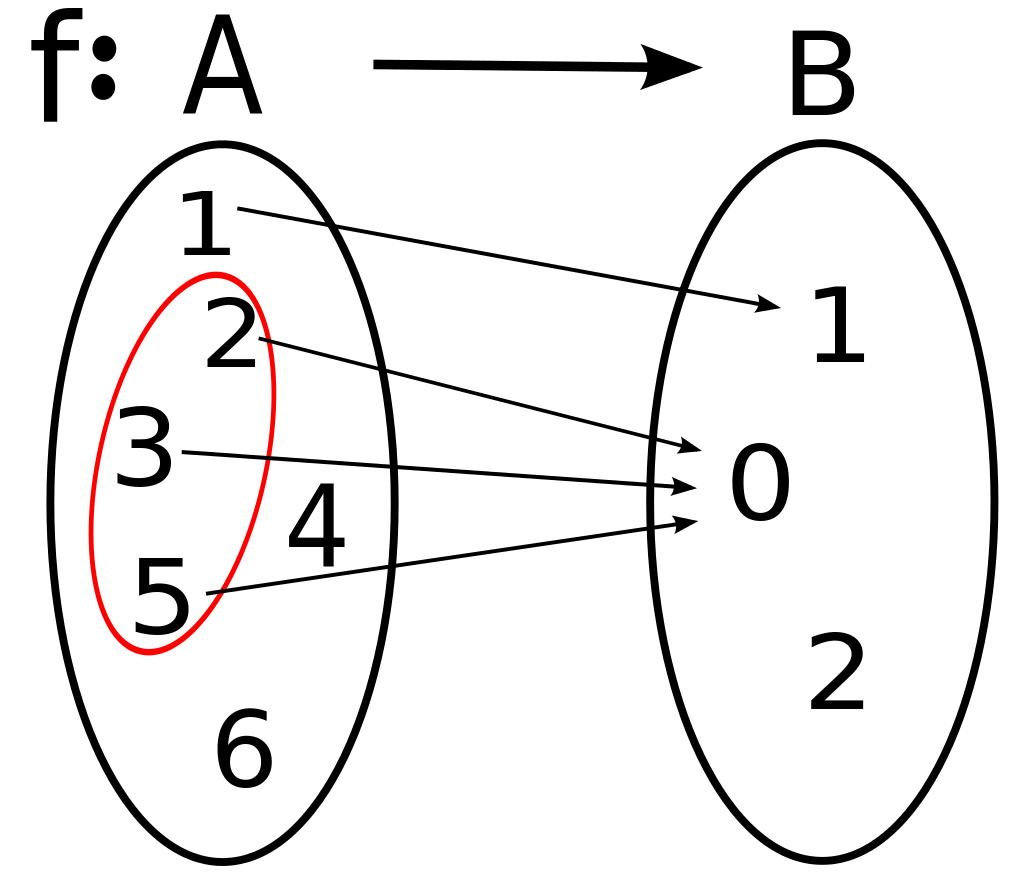
\includegraphics[width=0.4\textwidth]{../Bilder/urbild.png}
\label{urbild}
\caption{Beispiel: Das Urbild von $M=\{0\} \subset B$ ist $\{2,3,5\} \subset A$.}
\end{figure}

\section{$\sigma$-Algebra}
Sei $\Omega$ eine nichtleere Menge und $\mathcal{P}(\Omega)$ die Potenzmenge dieser Menge. Eine Menge von Teilmengen $\mathcal{A} \subset \mathcal{P}(\Omega)$ (auch Mengensystem genannt) heißt $\sigma$-Algebra auf, oder über $\Omega$, wenn sie die folgenden drei Bedingungen erfüllt:

\begin{enumerate}
	\item $\mathcal{A}$ enthält die Grundmenge, also: $\Omega \in \mathcal{A}$
	\item $\mathcal{A}$ ist stabil bezüglich der Komplementbildung. Ist also $A \in \mathcal{A}$, dann ist auch $A^{\mathrm{C}} \in \mathcal{A}$.
	\item $\mathcal{A}$ ist stabil bezüglich abzählbarer Vereinigungen. Sind also die Mengen $A_1, A_2, A_3, \dots$ in $\mathcal{A}$ enthalten, so ist auch $\bigcup_{i=1}^\infty$ in $\mathcal{A}$ enthalten.
\end{enumerate}

\section{Wahrscheinlichkeitsmaß}
Gegeben sei eine Menge $\Omega$, die Ergebnismenge und eine $\sigma$-Algebra $\Sigma$ auf dieser Menge (das Ereignissystem).\\

\noindent
Dann heißt eine Abbildung
\begin{equation}
P: \Sigma \rightarrow [0,1]
\end{equation}
Wahrscheinlichkeitsmaß, wenn sie die folgenden Bedinungen erfüllt.

\paragraph{Normiertheit:}
\begin{equation}
P(\Omega) = 1
\end{equation}

\paragraph{$\sigma$-Additivität:}
Für jede abzählbare Folge von paarweise disjunkten Mengen $A_1, A_2, A_3, \dots$ aus $\Sigma$ gilt
\begin{equation}
P\left( \bigcup^{\infty}_{i=1}A_i\right) = \sum_{i=1}^{\infty} P(A_i). 
\end{equation} 

\noindent
Es gilt also, dass die Wahrscheinlichkeit für die Vereinigung zweier Ereignisse gleich groß ist wie die Summe der Einzelwahrscheinlichkeiten der Ereignisse.

\section{Wahrscheinlichkeitsraum}
Sei $\Omega$ eine beliebige \textbf{Ergebnis}menge. Sie umfasst alle möglichen Ergebnisse von einem Zufallsvorgang. Beim Würfeln ergibt sich also beispielsweise $\Omega = \{ 1,2,3,4,5,6\}$.

\noindent
Nun wird $\Sigma$ als eine $\sigma$"=Algebra über $\Omega$ definiert. Die Elemente von $\Sigma$ werden auch Ereignisse genannt. 

\noindent
Als letztes wird ein Wahrscheinlichkeitsmaß $P: \Sigma \rightarrow [0,1]$ benötigt. Das Tripel $(\Omega, \Sigma, P)$ ist dann ein Wahrscheinlichkeitsraum.
 

\section{Messraum}
Ein Tupel $(\Omega, \Sigma)$ heißt Messraum, wenn $\Omega$ eine beliebige Grundmenge ist und $\Sigma$ eine $\sigma$-Algebra über $\Omega$ ist.

\noindent
In der Stochastik wird der Messraum auch Ereignisraum genannt und ist einfach ein Wahrscheinlichkeitsraum ohne Wahrscheinlichkeitsmaß.

\noindent
Eine Menge $S$ wird messbare Menge genannt, wenn $S \in \Sigma$ gilt.

\section{messbare Funktion}
Seien $(\Omega_1, \Sigma_1)$ und $(\Omega_2, \Sigma_2)$ zwei Messräume. Eine Funktion $f: \Omega_1 \rightarrow \Omega_2$ wird $\Sigma_1$"=$\Sigma_2$"=messbar genannt, wenn für alle $S_2 \in \Sigma_2$ gilt, dass das Urbild von $S_2$ unter $f$ ein Element aus $\Sigma_1$ ist:
\begin{equation}
f^{-1}(S_2) \in \Sigma_1.
\end{equation}

\noindent
\textit{In eigenen Worten: Aus Wahrscheinlichkeitssicht: Die Funktion $f$ bildet Ereignisse aus $\Omega_1$ auf Ereignisse in $\Omega_2$ ab. Wenn ich mir ein Ereignis $S_2$ aus $\Sigma_2$ nehme, also eine Teilmenge von $\Omega_2$, müssen alle Ergebnisse aus $\Omega_1$, die durch die Funktion $f$ auf Ergebnisse von $S_2$ abgebildet werden, zusammen ein Element von $\Sigma_1$ sein. \\
Das muss für alle $S \in  \Sigma_2$ gelten. Egal, welches Ereignis $S$ aus $\Sigma_2$ betrachtet wird, das Urbild von $S$ unter $f$ muss ein Element von $\Sigma_1$ sein. Zu jedem Element $S$ der $\sigma$"=Algebra $\Sigma_2$ muss es ein Element von $\Sigma_1$ geben, das das Urbild von $S$ unter $f$ ist.}






%\section{Übergangskern}
%Man hat zwei Messräume $(\Omega_0, \Sigma_0)$ und $(\Omega_1, \Sigma_1)$. Eine Abbildung $K: \Omega_0 \times \Sigma_1 \rightarrow [0, \infty)$ heißt Übergangskern von $(\Omega_0, \Sigma_0)$ nach $(\Omega_1, \Sigma_1)$, wenn gilt:

%$\bullet$ Für jedes $x \in \Omega_0$ ist $K(x,\ \cdot \ )$ ein Maß auf $(\Omega_1, \Sigma_1)$.

%$\bullet$ Für jedes $S \in \Sigma_1$ ist $K(\ \cdot \ , S)$ eine $\Sigma_0$-messbare Abbildung.



\end{document}